\section{Study 3: Evaluation on TypeBoard}

The motivations of study three were two-fold. First, we compared the performance and user experience of the TypeBoard and the ordinary touchscreen keyboard. Second, as we introduced in related work, tactile landmarks on keyboards improve users' typing speed by enabling touch typing, so we investigated the feasibility of TypeBoard plus tactile landmarks in this study. In summary, we evaluated users' typing performance on three settings: (1) ordinary software keyboard, (2) TypeBoard, and (3) TypeBoard plus, which was the TypeBoard plus tactile landmarks.

\subsection{Participants}

We recruited 15 participants from the campus (aged from 19 to 26, M = 20.87, SD = 2.42, seven females). All the participants were right-handed and did not take part in the previous studies. They have used software keyboards on smartphones for not less than two years (M = 6.67, SD = 2.06). Eleven participants have ever used software keyboards on tablets.

\subsection{Design and Procedure}

The study followed a within-subject design to compare users' typing speed in three keyboard configurations. The participant sat on an office chair. He could adjust the chair to a comfortable position. The participant typed on the pressure-sensitive touchpad to input words and received visual feedback from the tablet. As figure \ref{fig:study3_illu} shows, there were three keyboard settings in the experiment as follows:

\begin{enumerate}
	\item{\textbf{Config. 1):} \emph{Ordinary Keyboard.} On the ordinary software keyboard, all contacts on the touchscreen are recognized as keystrokes. Users need to hang their wrists in the air to avoid unintentional touches.}
	\item{\textbf{Config. 2):} \emph{TypeBoard.} TypeBoard is a software keyboard with unintentional touch rejection. The system only recognized intentional touches as keystrokes. Users can rest their hands on the keyboard.}
	\item{\textbf{Config. 3):} \emph{TypeBoard plus.} TypeBoard plus refers to the TypeBoard plus tactile landmarks. To provide tactile landmarks on TypeBoard, we attached 0.05 mm thick stickers on the touchpad to simulate physical keys. There were small bumps on the F and J keys, which is the same as the physical keyboard. Users could align their fingers without visual attention.}
\end{enumerate}

\begin{figure}[!tbh]
	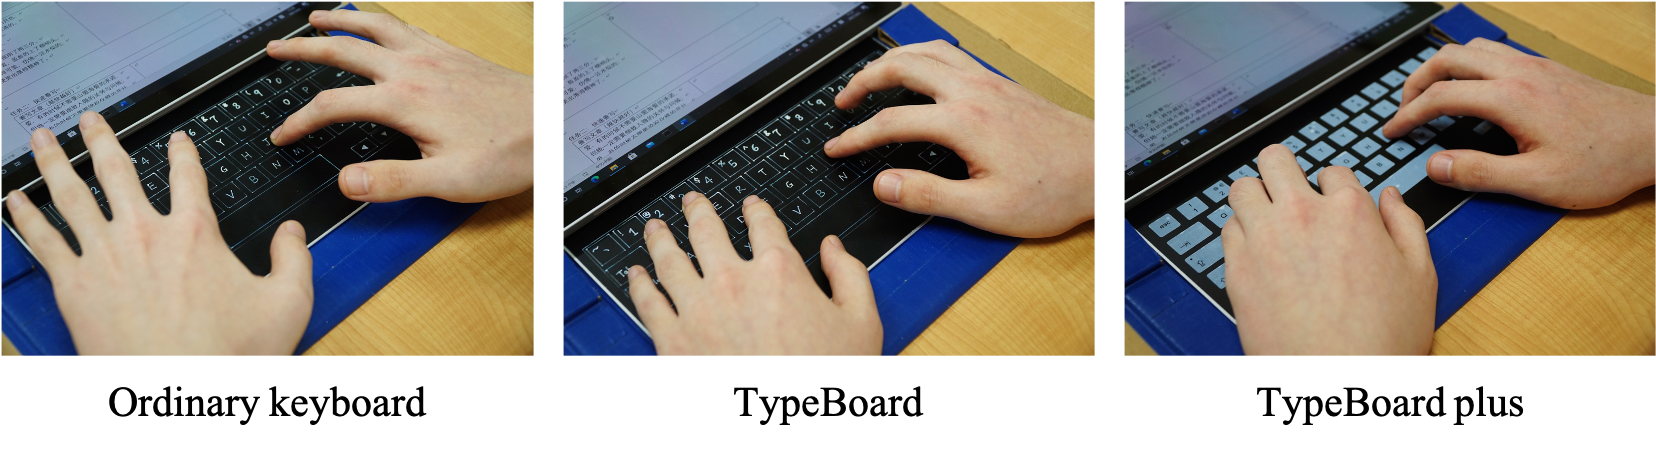
\includegraphics[width=1.0\linewidth]{figures/study3_illu.png}
	\centering
	\caption{The three keyboard settings in study three.}
	\label{fig:study3_illu}
\end{figure}

There were five sessions for each of the three keyboard configurations. In each session, participants transcribed a Chinese paragraph in a Microsoft Word document. There were roughly xx Chinese characters in a task paragraph. We randomly selected the task paragraphs in a typing speed measurement website \cite{Website-Typing}. Participants were asked to input as fast and accurately as possible. The transcription task is widely used in text entry researches \cite{2003-Metrics, 2003-Phrase, 2017-Word} to evaluate the ceiling typing speed.  We counterbalanced the order of keyboard configuration using a balanced latin square.
Participants had five minutes to warm up before they used each keyboard. They transcribed a paragraph to get familiar with the keyboard. The task phrases in the training step would not appear in the formal experiment. Participants rested for five minutes between sessions to avoid fatigue. On average, participants spent 90 minutes completing the experiment.

\subsection{Reslut}

A Repeated Measures (RM) ANOVA was conducted for text entry speed, Uncorrected Error Rate (UER), and Corrected Error Rate (CER). The within factors were the keyboard and the session. As UER and CER violated the normalcy, we used the Aligned Rank Transform \cite{2011-Aligned} for correction. If any independent variable had significant effects (p < 0.05), we used Bonferroni-corrected post hoc tests for pairwise comparisons.

\subsubsection{Speed}

We measured text entry speed in Chinese characters per minute (CPM). Participants used Pinyin \cite{Website-Pinyin}, a phonetic spelling system in Roman characters to input Chinese characters. To input a Chinese character, users type the Pinyin of the desired character (2 - 6 letters) and then select the target from a candidate list. Participants can also type the Pinyin of a Chinese word, consisting of two to four Chinese characters, and then select the whole word. In short, the process of inputting a Chinese character/word is similar to inputting an English word with word prediction/correction. We measured typing speed in CPM with this formula:

\begin{equation}
	CPM = \frac{|S|}{T} \times 60
\end{equation}

where |S| is the length of the transcribed paragraph in characters (including punctuation), and T is the completion time, i.e., the elapsed time in seconds from the first intentional touch to the last one. All the time consumption, including the time of candidate selection, was taken into account.

%我们使用的是中文输入法,我们所统计的量是中文字/分钟,公式是,当用户输入数字或字母时,其速度不纳入统计范围。我们测试了五种不同的输入任务,值得注意的是,只有transcription任务中的输入速度比较符合用户的ceiling speed,而在其它任务中,完成任务的时间包含了用户思考的时间和键鼠切换的时间。

\begin{figure}[!tbh]
	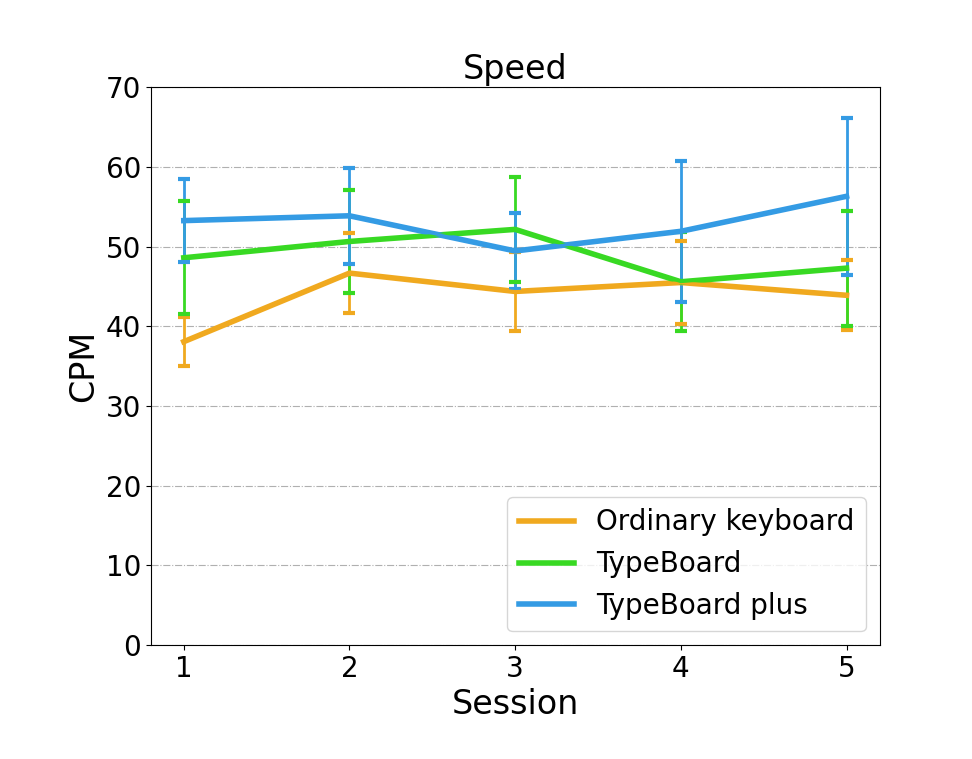
\includegraphics[width=0.6\linewidth]{figures/speed.png}
	\centering
	\caption{Text entry speed of the three keyboards over sessions. Error bars indicate 95\% confidence interval.}
	\label{fig:speed}
\end{figure}

Figure \ref{fig:speed} shows the users' typing speeds over sessions. There is no significant effect of session on speed ($F_{4,56}=1.76,p=.15,\eta_p^2=0.11$). The result indicates that the learning costs of the three keyboards were low. Participants reached the ceiling performance after a five-minute training. Keyboard has a significant effect on speed ($F_{2,28}=26.76,p<.001,\eta_p^2=0.66$). Pair-wise comparisons show significant differences between all the keyboard pairs: ordinary keyboard vs. TypeBoard ($p<.005$), ordinary keyboard vs. TypeBoard plus ($p<.001$), and TypeBoard vs. TypeBoard plus ($p<.005$). The participants' average typing speed on the ordinary keyboard was 43.71 CPM (SD = 6.52). The typing speed on the TypeBoard was 48.87 CPM (SD = 10.14), outperforming the ordinary keyboard by 11.78\%. The typing speed on the TypeBoard plus was 52.97 CPM (SD = 9.85), outperforming the ordinary keyboard by 21.19\%. Results show that the TypeBoard improves the efficiency of the touchscreen keyboard.

\subsubsection{Error rate}

We used two metrics to measure text entry accuracy: (1) Uncorrected Error Rate (UER) - text entry errors that remain in the transcribed string. UER is the number of uncorrected erroneous Chinese characters divided by the number of correct and erroneous characters. (2) Corrected Error Rate (CER) - text entry errors that are fixed (e.g., backspaced) during entry. CER is the number of corrected erroneous Chinese characters divided by the number of correct and erroneous characters. The corrections of Pinyin while inputting a word were not taken into account of CER. As UER and UER violated the normalcy, we used the Aligned Rank Transform for nonparametric factorial analysis \cite{2011-Aligned}.

\begin{figure}[!tbh]
	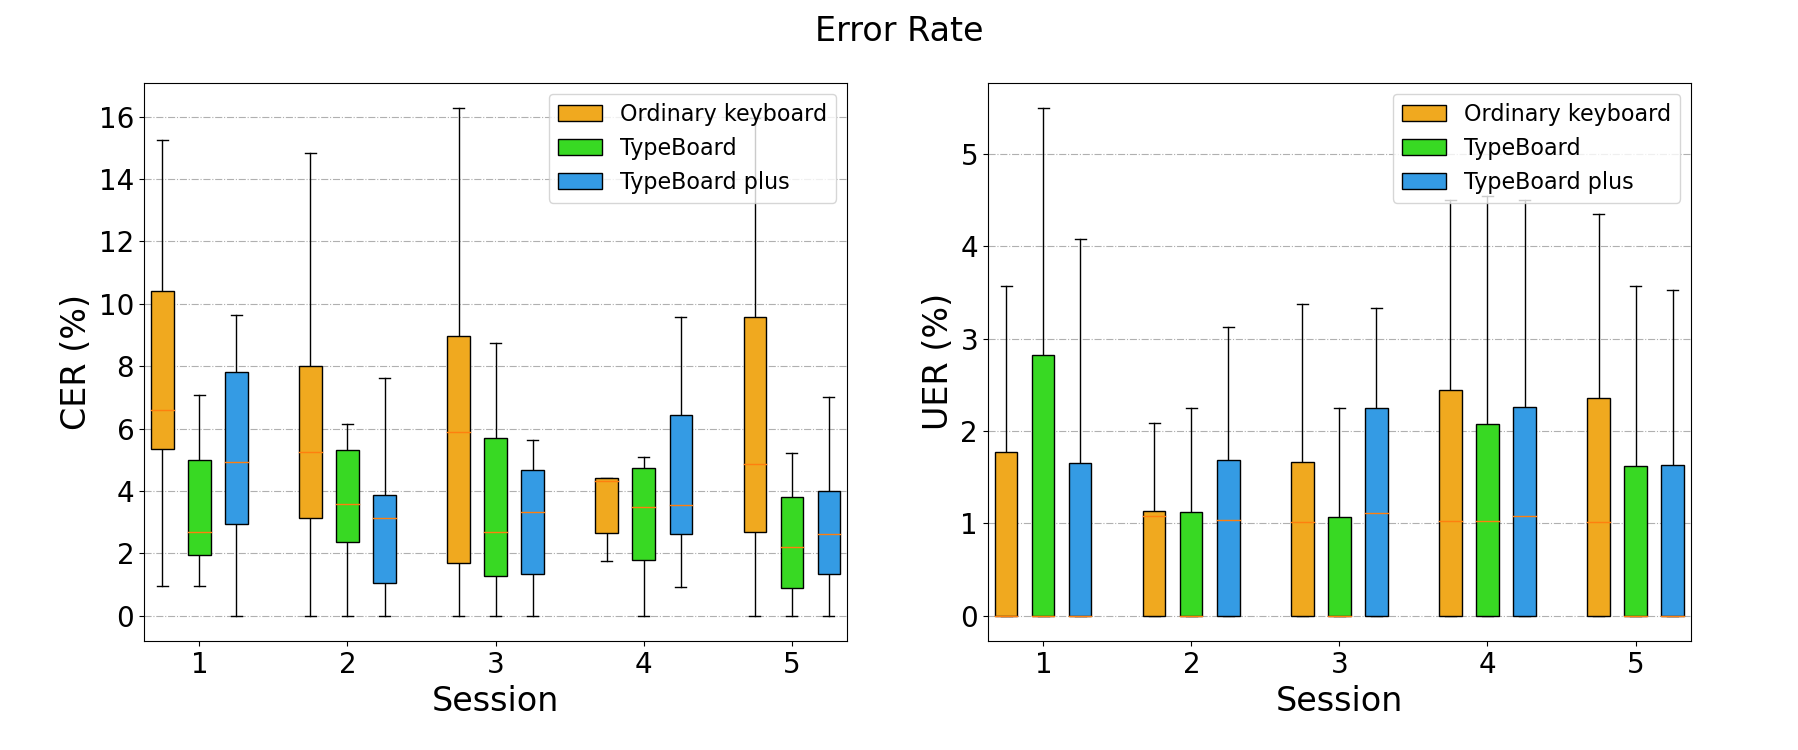
\includegraphics[width=1.0\linewidth]{figures/error_rate.png}
	\centering
	\caption{Uncorrected error rates and Corrected error rates of the three keyboards over sessions.}
	\label{fig:error_rate}
\end{figure}

Figure \ref{fig:error_rate} shows the CER and the UER over sessions. There is no significant effect of session on CER ($F_{4,56}=1.01,p=.39$). Keyboard has a significant effect on CER ($F_{2,28}=9.49,p<.005$). Pair-wise comparisons showed significant differences between the following keyboard pairs: ordinary keyboard vs. TypeBoard ($p<.01$), and ordinary keyboard vs. TypeBoard plus ($p<.005$). The average CERs of the ordinary keyboard, TypeBoard, and TypeBoard plus were 6.66\% (SD = 4.42\%), 4.58\% (SD = 3.58\%), and 4.21\% (SD = 2.58\%).
There is no significant effect of session ($F_{4,56}=0.41,p=.71$) or keyboard ($F_{2,28}=0.001,p=.998$) on UER. The average UERs of the ordinary keyboard, TypeBoard, and TypeBoard plus were 1.29\% (SD = 1.67\%), 1.28\% (SD = 1.38\%), and 1.28\% (SD = 1.16\%).
Results show that the TypeBoard reduces the probability of making typos compared with the ordinary keyboard. This is the main reason the TypeBoard improves the typing speed of the touchscreen keyboard. The TypeBoard plus does not reduce the probability of making a typo compared with the TypeBoard. Thus, there are other reasons for faster typing on the TypeBoard plus.

%在中文输入法中,CER可能会比其它语言的输入法更多,这是因为用户可能会利用词语的联想功能来打一个汉字,然后把后面那个字删掉。

%Figure 14 shows the UER and the CER over five days. There is no significant effect of model or day on UER. The average UER was 1.17% (SD = 1.02%) for the general model and 1.50% (SD = 1.40%) for the personal model. There is no significant effect of the model on CER. The days have a significant effect on CER (F4,56 = 6.84,p < .005). Pair-wise comparisons showed significant differences between the following day pairs: 1-3(p<.005), 1-4(p<.05), 1-5(p<.005), 2-3(p<.05) and 2-5(p<.05). On day 5, the average CER was 3.22% (SD = 2.92%) for the general model and 2.92% (SD = 1.65%) for the personal model. That is, participants made corrections once every 30 words with both of the models.

\subsubsection{Time components}

To gain deeper insight into the performance comparison among keyboards, we broke down the text entry time into four components: typing time, selecting time, deleting time, and pause time. Typing time was the time spent on typing Pinyin. Selecting time was the time spent on selecting a candidate Chinese character/word. Deleting time was the time spent on deleting characters. Pause time span from inputting the last character/word to starting the next character/word. Figure \ref{fig:time_components} shows the typing time, selecting time, deleting time, and pausing time per Chinese character over the three keyboards. RM ANOVAs showed that keyboard has significant effects on selecting time ($F_{2,28}=7.85,p<.005$), deleting time ($F_{2,28}=20.89,p<.001$), and pause time ($F_{2,28}=12.76,p<.001$).
Pair-wise comparisons showed that both the TypeBoard (p<.001) and the TypeBoard plus (p<.001) reduce the ordinary keyboard's deleting time. The results showed that unintentional touch prevention reduced typos.
The TypeBoard plus significantly reduced the pause time compared to the ordinary keyboard (p<.001) and the TypeBoard (p<.005). The results indicated that participants performed touch typing more frequently on the TypeBoard plus, saving the time of finding the next transcribing word.

\begin{figure}[!tbh]
	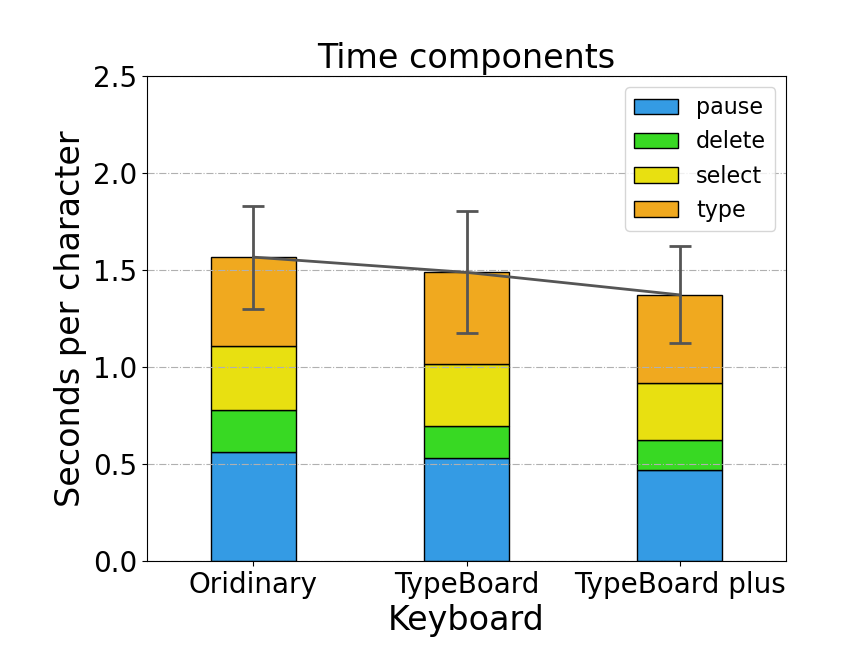
\includegraphics[width=0.6\linewidth]{figures/time_components.png}
	\centering
	\caption{Time components.}
	\label{fig:time_components}
\end{figure}

%\subsubsection{Unintentional touches}
%For the three configurations ordinary keyboard, TypeBoard and TypeBoard plus, the proportions of unintentional touches were xx.xx\%, xx.xx\% and xx.xx\% respectively.

\subsubsection{Touch position}

Figure \ref{fig:touch_position} shows the distribution of intentional touches on the TypeBoard and the TypeBoard plus . For convenience, we assumed that the point clouds obeyed 2D Gaussian distributions. While the key width is xx mm and key height is xx mm, the average X/Y offsets were xx/xx mm on the TypeBoard and xx/xx mm on the TypeBoard plus. This result shows that users tend to touch shift towards the xx of the keyboard. The average X/Y standard deviations of the distributions were xx/xx mm and xx/xx mm on the two keyboards. An paired sample t-test shows that keyboard has a significant effect on the average product of X and Y standard deviations (F, p), which indicated that users typed more accurately on the TypeBoard plus (p<). Users touched the tactile landmarks on the TypeBoard plus to aligned their fingers, which improved the typing accuracy.

\begin{figure}[!tbh]
	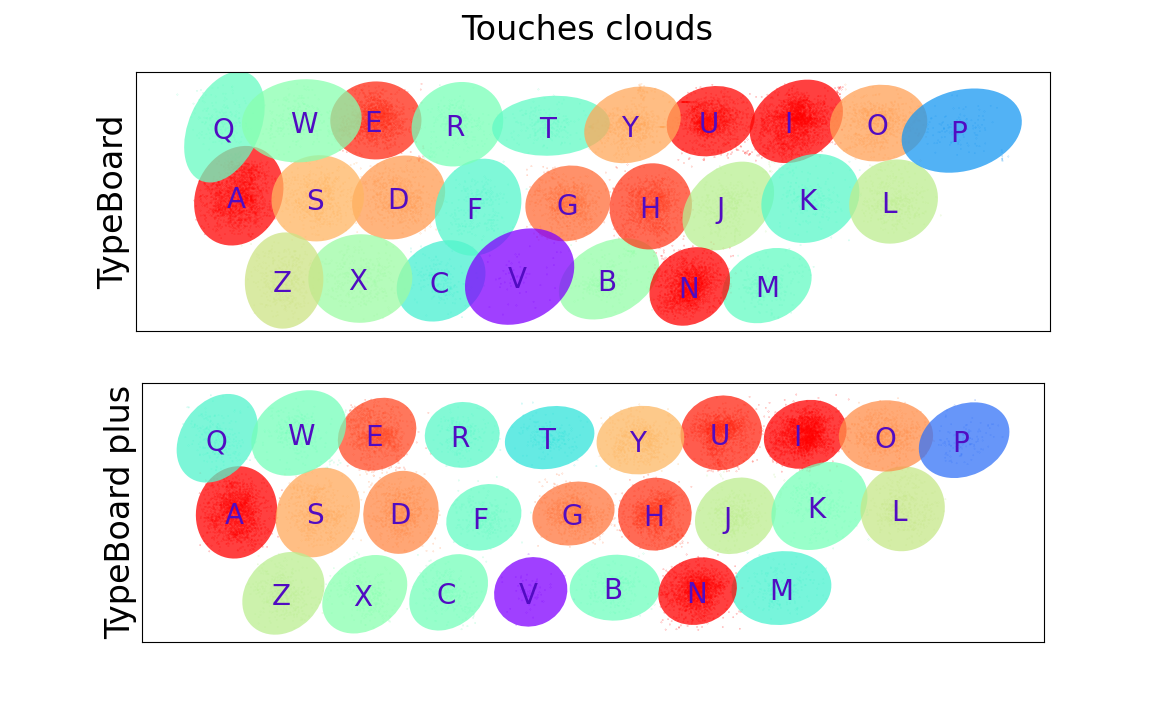
\includegraphics[width=0.8\linewidth]{figures/touch_position.png}
	\centering
	\caption{The distributions of intentional touches on the TypeBoard (above) and the TypeBoard plus (below). The ellipses show 1 standard deviation of the distribution.}
	\label{fig:touch_position}
\end{figure}

\subsubsection{Subjective Rating and Feedback}

Participants rated the subjective speed, accuracy, fatigue, and cognitive load on a 7-point Likert scale (1 - the worst; 7 - the best) after using each keyboard. Figure \ref{fig:subjective_feedback} shows the results. Wilcoxon Signed-Rank tests show that the TypeBoard significantly improves the ordinary keyboard's subjective speed ($Z=-2.27,p<.05$), accuracy ($Z=-3.24,p<.005$), fatigue ($Z=-2.84,p<.005$), and cognitive load ($Z=-1.99,p<.05$). The TypeBoard plus improves the ordinary keyboard's subjective speed ($Z=-3.17,p<.005$), accuracy ($Z=-3.52,p<.001$), fatigue ($Z=-3.34,p<.001$), and cognitive load ($Z=-2.28,p<.05$). The TypeBoard plus is better than the TypeBoard on subjective speed ($Z=-2.40,p<.05$) and fatigue ($Z=-2.85,p<.005$). Results show that both the TypeBoard and the TypeBoard plus improve the ordinary keyboard's user experience.

\begin{figure}[!tbh]
	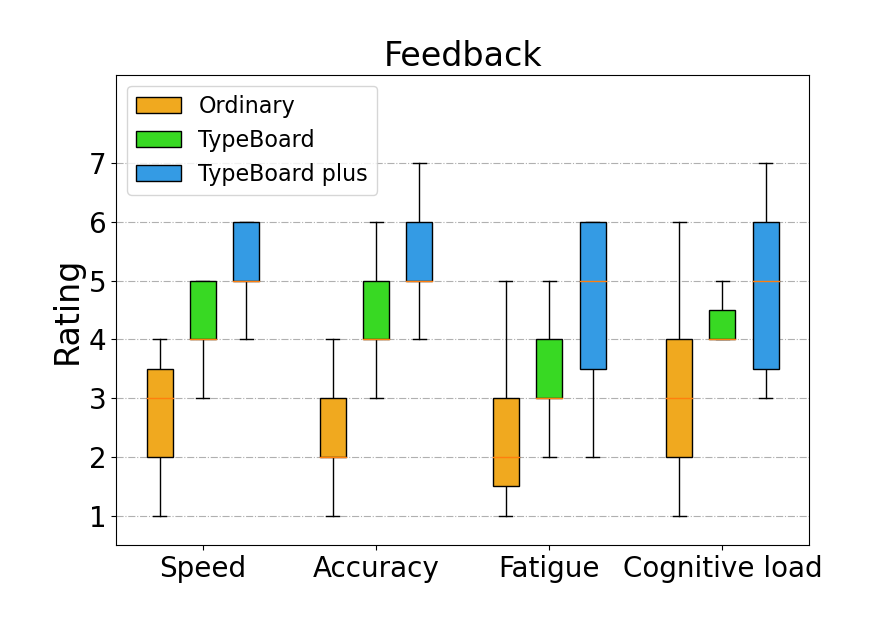
\includegraphics[width=0.6\linewidth]{figures/subjective_feedback.png}
	\centering
	\caption{Subjective ratings (higher is better).}
	\label{fig:subjective_feedback}
\end{figure}

\subsection{Summary}

\subsubsection{Ordinary Keyboard vs. TypeBoard}

The TypeBoard improves the ordinary tablet keyboard's typing speed by 11.78\%. The TypeBoard has the advantages of avoiding fatigue, relieving cognitive load, and reducing typos.

\subsubsection{TypeBoard vs. TypeBoard plus}

The TypeBoard plus further improve the TypeBoard's typing speed by 8.51\%, outperforming the ordinary tablet keyboard by 21.19\%. Compared to the TypeBoard, the TypeBoard plus has the advantages of improving typing accuracy and reducing pause time.
